\documentclass[10pt,conference,compsocconf]{IEEEtran}

%\usepackage{times}
%\usepackage{balance}
\usepackage{url}
\usepackage{graphicx}	% For figure environment
\usepackage{color}
\usepackage{subcaption}
\usepackage{hyperref}

\newcommand{\todo}[1]{{\color{red}{\textbf{TODO: #1}}}}
\newcommand{\conv}[3]{$ \cal{C} $(#1$ \times  $#1, #2, #3)}
\newcommand{\relu}{$ \cal{R}~$}
\newcommand{\maxpool}[2]{$ \cal{M} $(#1$ \times $#1, #2)}
\newcommand{\lrn}{$ \cal{LRN}~$}
\newcommand{\fc}[2]{$ \cal{FC} $(#1, #2)}

\begin{document}
\title{Road Extraction from Aerial Images}
\author{
  Delio Vicini, Matej Hamas, Taivo Pungas\\
  Department of Computer Science, ETH Zurich, Switzerland
}

\maketitle

\begin{abstract}
  TODO - last
\end{abstract}

\section{Introduction}
\label{sec:intro}

In this paper, we present a novel technique for detecting roads on aerial images. The solution to this problem has potentially many application ranging from automation of map making to urban planning and environmental monitoring.

Given an RGB aerial or satellite image of a moderate resolution, we seek to classify each 16x16 patch as \textit{road} or \textit{non-road}. Hence, this is an instance of a binary classification problem.

As this is quite long-standing problem in computer vision, and thanks to its many applications, there is rich previous work in this area \cite{Huang.2002} \cite{MnihThesis.2013} \cite{Long.2014} \cite{Montoya.2015} \cite{Saito.2015}. Most of the past work concentrated on per-pixel prediction from aerial images. Some papers also look at multi-class semantic classification by introducing specific \textit{building} class \cite{Saito.2015}. 

Previous approaches include support vector machines (SVMs) on manually extracted features \cite{Huang.2002}, convolutional neural networks (CNNs) \cite{Long.2014} \cite{Saito.2015}, conditional random fields \cite{Montoya.2015} and other probabilistic approaches.

Unlike most of the previous work, we concentrate on per-patch and not on per-pixel prediction. We have developed a novel solution by combining a deep CNN with an SVM based post-processing.

We compare our approach to two different baseline algorithms. One of them is a plain vanilla 2-layer CNN with SGD optimizer. The second is the same CNN followed by a denoising step by means of dictionary filtering.

In conclusion, our main contributions are patch-based, \mbox{4-layer} CNN architecture for road segmentation followed by the SVM based post-processing scheme. 

\begin{figure}[]
	\centering
	\begin{subfigure}{.2\textwidth}
		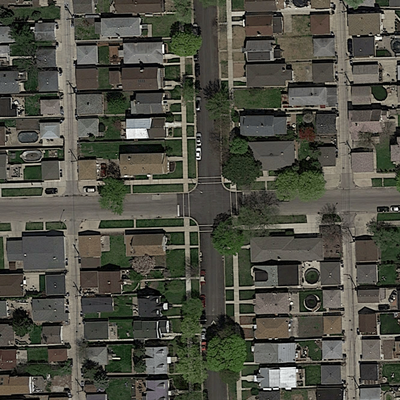
\includegraphics[width=1\textwidth]{figs/img1.png}
	\end{subfigure}
	\begin{subfigure}{.2\textwidth}
		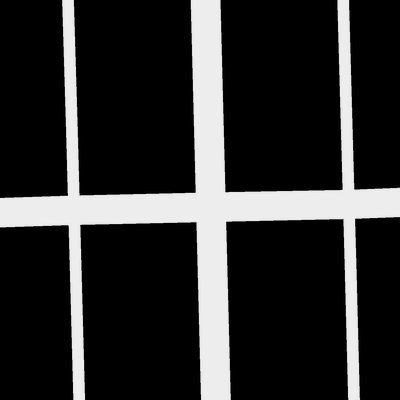
\includegraphics[width=1\textwidth]{figs/groundtruth1.png}
	\end{subfigure}
	\caption{Aerial image of an urban scene and the ground truth showing the road.}
\end{figure}

\section{Models and Methods}
\label{sec:MM}
In this section we will describe data augmentation techniques, baseline and final CNN architectures and post-processing techniques applied on the top of the CNN output.

\subsection{Data Augmentation}
\label{subsec:preprocessing}
The lack of training data is a universal problem in machine learning. To maximize both the quantity and quality of our training data, we have implemented a sliding window approach which extract patches of a particular size from input images. To enlarge the dataset, we generate more training patches by flips and rotations.

Afterwards, we zero-mean the training dataset by subtracting the mean image from all patches. We do not divide by standard deviation as the images are naturally well distributed.

We then generate the corresponding ground truth labels from the input images by the same sliding window procedure, followed by the thresholding with a threshold 0.25. The labels are stored in a 1-hot format, i.e. as tuples [0, 1] or [1, 0].

Finally, we balance the training dataset to include the same number of [0, 1] and [1, 0] examples. This is done to prevent a potential bias learnt by the CNN.

\subsection{Notation - CNN Architecture}
Here, we provide a short overview of possible CNN layers that are used in the following sections.
\begin{itemize}
	\item \conv{N}{I}{O} \\
	Standard convolutional layer with filters of size N$ \times $N, I input channels and O outputs channels. The default stride is 1 both vertically and horizontally and the image is padded so it retains the size.
	\item \maxpool{N}{S} - Max-pooling layer of size N$ \times $N, stride S.
	\item \lrn - Local response normalization layer across the current batch \cite{tensorflow.2015}.
	\item \fc{I}{O} - Standard fully connected layer from I input channels to O output channels.
\end{itemize}

\subsection{Baseline CNN Architecture}
\label{subsec:baselineCNN}
The baseline CNN operates on patches of size $16 \times 16$. It has two convolutional and two fully connected layers with the following architecture:
\begin{center}
	\conv{5}{3}{32} -- \conv{5}{32}{64} -- \\ 
	\fc{1024}{512} -- ReLU -- \fc{512}{2}.
\end{center}
ReLU and \maxpool{2}{2} is applied after every convolutional layer.

The activation functions in the $ \cal{FC} $ layers are identities. We apply \textit{softmax} to two outputs to get the probabilities for both classes. All the weights are initialized normally with standard deviation 0.1. The weights in the $ \cal{FC} $ layers are L2 regularized with a factor $ 5 \times 10^{-4} $. We use a plain vanilla SGD optimizer with an exponentially decaying learning rate, starting at 0.01 with a decay rate 0.95. Batch size is 16. 

\subsection{Final CNN Architecture}
\label{subsec:CNN}
We have been tweaking the baseline CNN in various ways to improve its performance. We made it deeper, experimented with the widths of layers and filter sizes, tried using dropout or local response normalization instead of L2 regularization of $ \cal{FC} $ weights, tested different optimizers (momentum and Adam) and learning rates. We also implemented cross-validation to estimate the training time after which the out-of-sample error converges.

Moreover, we increased the context size to $ 64\times64 $, i.e. the network predicts a label for the central $ 16\times16 $ patch using larger context. Boundaries are mirrored.

The final architecture of the 4-layer CNN is the following:
\begin{center}
	\conv{5}{3}{16} -- \conv{3}{16}{32} -- \\ 
	\conv{3}{32}{32} -- \conv{3}{32}{64} -- \\
	\fc{1024}{64} -- ReLU -- \fc{64}{2}.
\end{center}
After every convolutional layer, we apply ReLU, \lrn and \maxpool{2}{2}.

The activation functions in the first $ \cal{FC} $ layer are identities and in the second sigmoids. We use neither dropout, nor L2 regularization of the $ \cal{FC} $ weights. The class probabilities are again obtained using \textit{softmax}.

After discovering that exponential decaying learning rate does not help, we have fixed it to the empirically determined value 0.01. 
In the final model, we use Adam optimizer with $ \epsilon = 0.1 $ and the batch size is 32. All the weights are initialized normally using standard deviation 0.1.


\subsection{Postprocessing}
The convolutional neural network outputs independent predictions for all $ 16 \times 16 $ patches of the processed image. The spatial arrangement of predictions however contains valuable information, which can be used to further improve the prediction accuracy. For example, it is highly unlikely to observe a road which only covers one patch. If the CNN predicts an isolated patch as belonging to the road label, we can discard this prediction with high certainty. The opposite also holds: a patch labeled as non-road surrounded by patches labeled as road is most likely part of the road as well. Oftentimes false negatives are caused by shadows or overlapping structures such as railway bridges.

\par 
In our algorithm, we filter the CNN output by predicting the label of a patch from the labels of the surrounding patches. Given a window of $ 7 \times 7 $ patches predicted by the CNN, we predict the label of the central patch using a binary support vector machine (SVM) classifier. We directly use the probabilities produced by the CNN as features for the SVM classifier. We also tried to automatically extract features using Restricted Boltzmann Machines \cite{smolensky.1986}, but could not achieve an increase in prediction accuracy.
\par
The SVM uses a radial basis function kernel and a soft-margin penalization weight of $ 1 $. We did not perform a systematic search for optimal SVM hyper-parameters, as these parameters seem to work reasonable well.
\par 
We found it beneficial to iteratively apply this denoising technique. This seems to help to propagate confident predictions. In practice, we use only two iterations. After two iterations most noise is already removed. Increasing the number of iterations biases the predictions too much and does not lead to a gain in accuracy.

\par
An alternative method to remove noise from the predictions is to use learned dictionaries \cite{Elad.2006}. We found this to work quite well if the level of noise in the CNN predictions is high. However, as the quality of the CNN improves, dictionary based denoising becomes less useful. We also tried using graph cut based inference \cite{Boykov.2001}. For this we computed per-pixel labels by accumulating per-pixel votes using a sliding window. This however did not work well, since graph cut based image segmentation relies on strong edges between fore- and background. In our aerial images, this is not the case and the boundary between road and non-road is fairly weak in terms of local edge contrast.

\todo{also describe simple neighborhood filtering}

\section{Results}
\label{sec:results}
The neural network was implemented using Tensorflow \cite{tensorflow.2015} and the post processing using scikit learn \cite{sklearn.2011}. Our CNN model trains for around 20 hours on a cluster node with  \todo{HARDWARE} (on the CPU) and the post processing SVM trains for around 1.5 hours. Individual satellite images are processed in a matter of seconds.

\par 
We compare our method to two different baseline implementations. The first is the CNN described in \todo{REFER TO SECTION}. In the following we refer to this implementation as \emph{CNN1}. The second one is the same CNN combined with dictionary based denoising, called \emph{CNN1Dict} in the following. We measure model accuracy as the reported score in the public Kaggle leader board. The model CNN1 achieves an accuracy of only \todo{percent}. Post processing the output from this networks improves the accuracy to \todo{percent} percent. 

\par
Our improved CNN on its own achieves an accuracy of  \todo{percent}. Applying our SVM based post processing procedure on top of these outputs, we get an accuracy of around  \todo{percent}.

\section{Discussion}
\label{sec:discussion}
TODO

\section{Summary}
\label{sec:summary}
TODO - last

\section*{Acknowledgements}
TODO

\bibliographystyle{IEEEtran}
\bibliography{references}
\end{document}
